In order to reduce the overlap with other \gls{atlas} data analyses, especially
those containing multijet final states, an upper cut on the number of \gls{hs}
jets is necessary. This procedure is denominated \emph{jet veto}. In order to
define hard scatter jets, cuts on the jet $\pt$ and on the \gls{jvt} (see
\cref{sec:jet-vertex-tagger}) have been studied. The aim of these cuts is to
render the analysis independent from pile-up as much as possible but stay signal
efficient, too hard cuts would lead to disregarding possible signal events
while, on the other hand, too loose cuts let pile-up jets in the signal region
and allow significant overlap with other \gls{atlas} searches.

Due to the jets coming from the squark decays, the \gls{susy} compressed
squark-neutralino model has more jets compared to other signals considered in
the monojet analysis and are therefore the most sensitive to jet veto efficiency
and to the definition of hard scatter jet. To study the pile-up contamination
for different $\pt$ thresholds a \emph{figure of merit} is defined and its
dependence from the average number of proton-proton collisions per bunch
crossing studied. The figure of merit is referred to as \emph{jet veto
  efficiency } and defined as:
\begin{equation}
  \label{eq:fig_merit}
  \frac{\text{N (events) with baseline cuts + at
      most N (jet) HS jets}}{\text{N (events)
      with baseline cuts}}
\end{equation}
where the baseline cuts are the event selection given in
\cref{sec:event-selection} except the cut F (the study presented here uses a
symmetric $\met$ and leading jet $\pt$ cut at 250~GeV) and the hard scatter jets
are defined as:
\begin{itemize}
\item Jets with $\pt > 50$ GeV is always considered coming from the hard
  scatter.
\item Due to the lacking of a tracking system in the $|\eta| > 2.4$ region and
  thus the impossibility of using a \gls{jvt} criteria, jets belonging to the
  $|\eta| > 2.4$ (forward jets) are always considered as coming from the hard
  scatter.
\item In order to be considered coming from the hard scatter proton-proton
  collision, the jets with $\pt^{\mathrm{thresh}} < \pt < 50$~GeV must
  additionally satisfy a
  $\mathrm{\gls{jvt}}~>~\mathrm{\gls{jvt}}^{\text{ thresh}}$ selection criteria
  where different $\pt^{\mathrm{thresh}}$ and \gls{jvt}$^{\mathrm{\, thresh}}$
  are studied, in particular:
  \begin{enumerate}[A -]
  \item
    $\pt^{\mathrm{thresh}} \in
    \{30~\mathrm{GeV},~40~\mathrm{GeV},~50~\mathrm{GeV}, ~70~\mathrm{GeV}\}$,
  \item \gls{jvt}$^{\mathrm{\, thresh}}~\in~ \{0.14,~0.64,~0.92\}$.
  \end{enumerate}
\end{itemize}

As can be seen from \cref{fig:susy_compressed}, at least three jets in the event
are required for the \gls{susy} compressed spectra models, on the other hand
other searches~\cite{MultijetSUSY} already explore signatures with four jets or
more. For these reasons and to increase the acceptance of the \gls{susy}
compressed models, events with at most three or four jets are studied with
different $\pt$ thresholds.  \cref{fig:comp_4jets_nojvt,fig:comp_3jets_nojvt}
shows the jet veto efficiency for the different values of
$\pt^{\mathrm{\, thresh}}$ and number of jets in the case where no \gls{jvt} cut
is applied. With a maximum number of jets of three 30~GeV jets the signal
efficiency loss is as large as 20\%. The \gls{jvt} cut reduces the loss of
efficiency for the signal, by preventing pile-up jets to trigger a veto of the
signal events. For three jets at 30~GeV the loss of signal is reduced from about
20\% in \cref{fig:comp_3jets_nojvt} to approximately 15\% in
\cref{fig:comp_3jets_jvt64} and becomes lesser than 5\% for at most four jets.
% \cref{fig:comp_4jets_nojvt} shows the jet veto efficiency for the
% different values of $\pt^{\mathrm{\, thresh}}$ and N~(jets)~$\leq~4$ in the case
% where no JVT cut is applied. In the case of $\pt^{\mathrm{\, thresh}}$ of 30~GeV
% the pile-up dependence is noticeable while it becomes less important with
% tighter cuts. In \cref{fig:comp_4jets_jvt64} a JVT $>$ 0.64 selection is applied
% in the definition of the hard scatter jets, in this case the pile-up dependence
% for the $pt^{\mathrm{\, thresh}}$ of 30~GeV is reduced and the distribution for
% $\pt^{\mathrm{\, thresh}}$ of 40, 50 and 70~GeV cuts is, within statistical
% error, flat.
\begin{figure}[!h]
  \centering
  \begin{subfigure}[t]{.48\linewidth}
    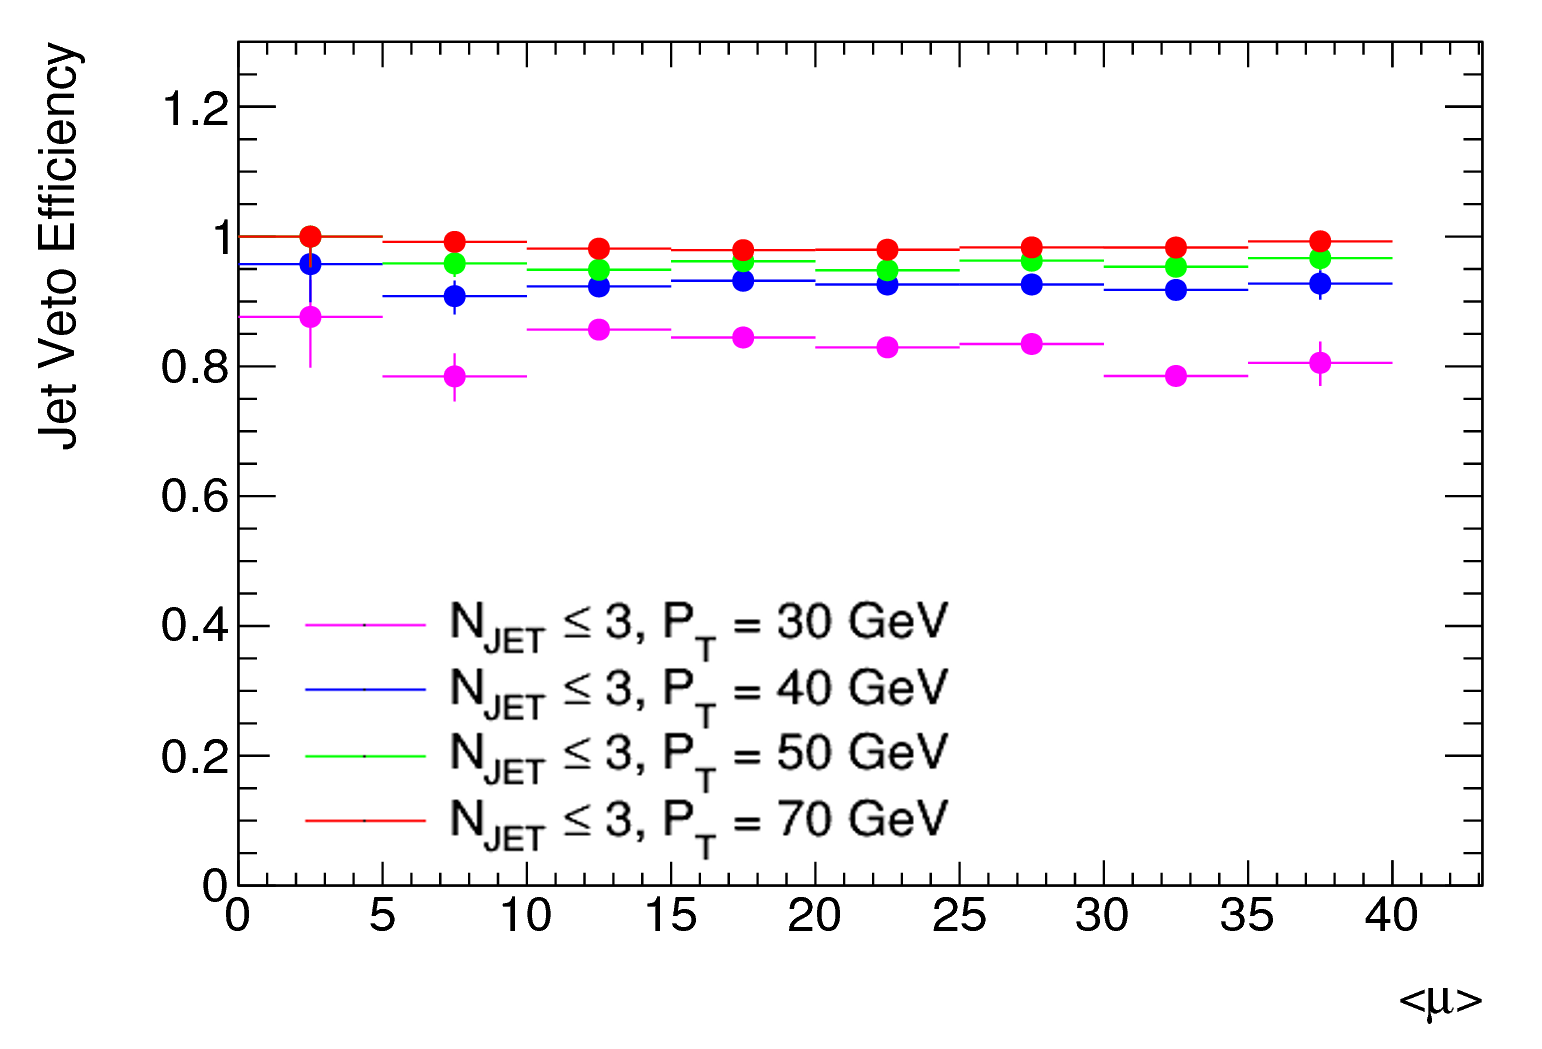
\includegraphics[width=\linewidth]{Compressed_450_435_mu_3jets_M0}
    \caption{No JVT cut applied.}
    \label{fig:comp_3jets_nojvt}
  \end{subfigure}
  \begin{subfigure}[t]{.48\linewidth}
    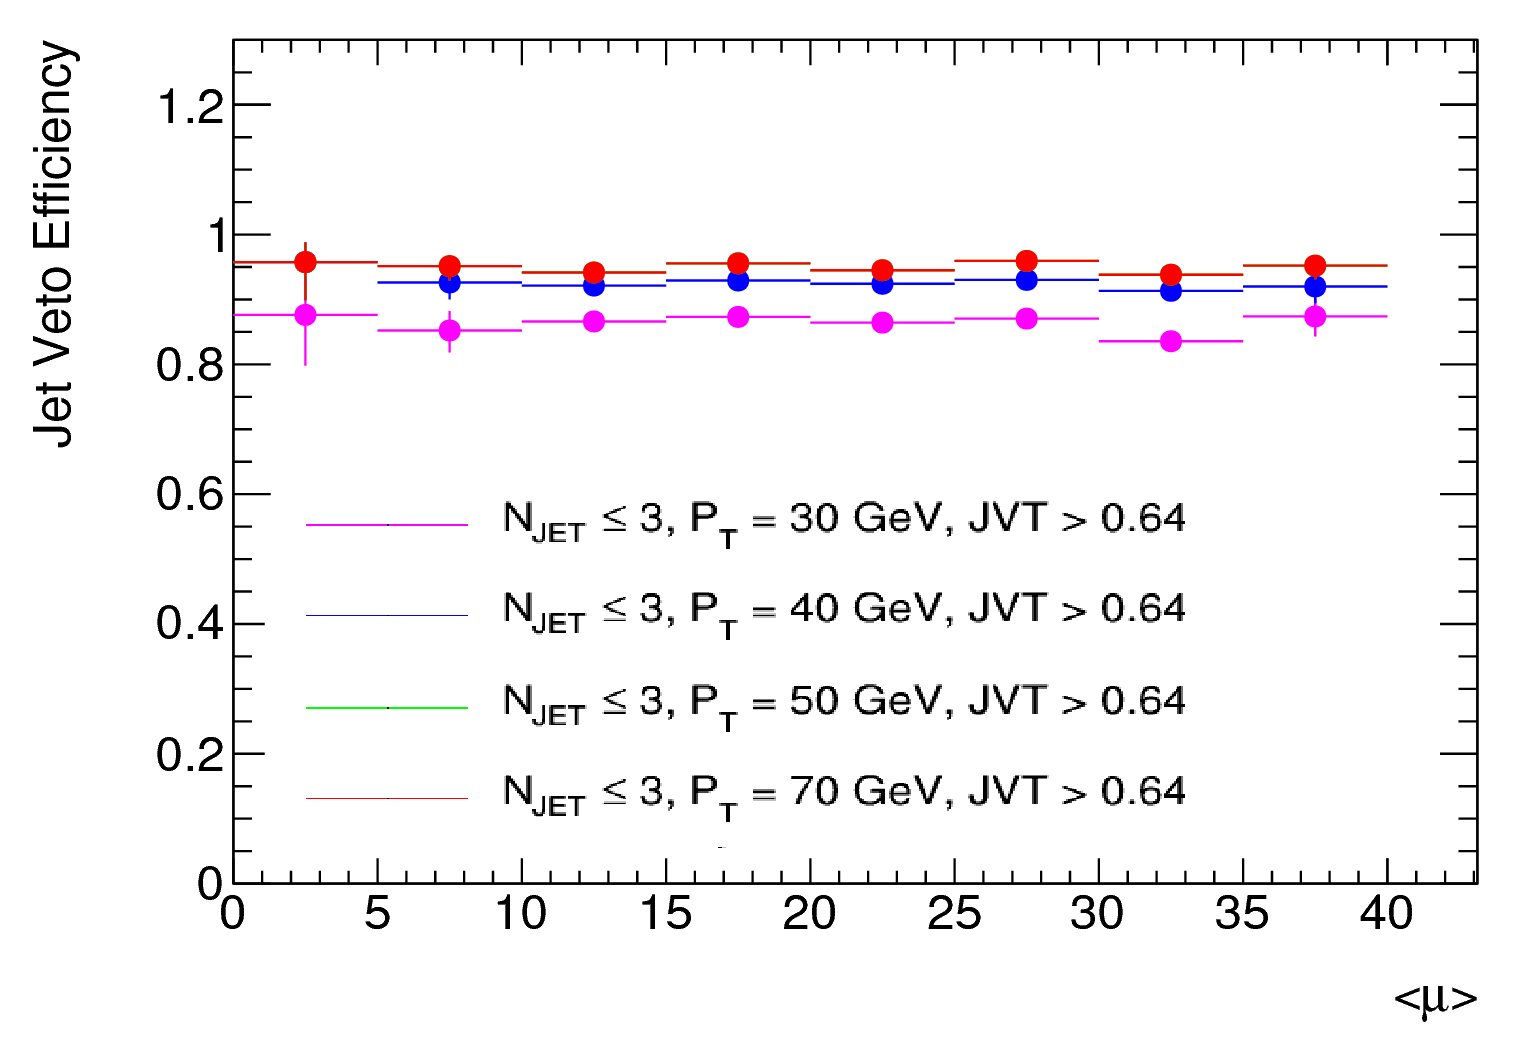
\includegraphics[width=\linewidth]{Compressed_450_435_mu_3jets_jvt64_M0}
    \caption{JVT > 0.64.}
    \label{fig:comp_3jets_jvt64}
  \end{subfigure}
  \begin{subfigure}[t]{.48\linewidth}
    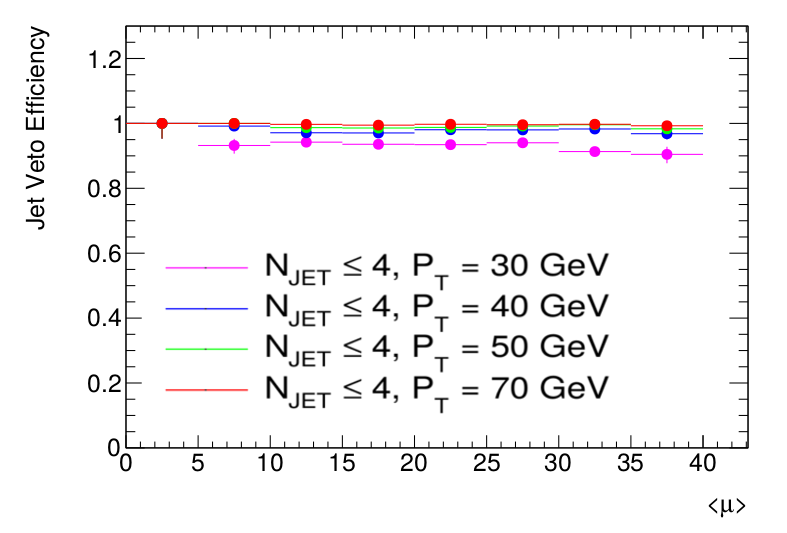
\includegraphics[width=\linewidth]{Compressed_450_435_mu_4jets_M0}
    \caption{No JVT cut applied.}
    \label{fig:comp_4jets_nojvt}
  \end{subfigure}
  \begin{subfigure}[t]{.48\linewidth}
    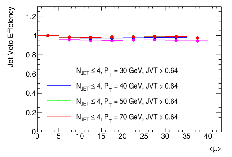
\includegraphics[width=\linewidth]{Compressed_450_435_mu_4jets_jvt64_M0}
    \caption{JVT > 0.64.}
    \label{fig:comp_4jets_jvt64}
  \end{subfigure}
  \caption{Jet veto efficiency for different jet $\pt$ thresholds and number of
    jets as a function of the average number of interactions per bunch crossing
    $\langle \mu \rangle$ for a compressed spectra model point $\msquark = 450$
    GeV $\mneutralino = 435$ GeV. In
    \cref{fig:comp_4jets_nojvt,fig:comp_3jets_nojvt,} no \gls{jvt} cut is
    applied and there is some drop of the efficiency at high pile-up. In
    \cref{fig:comp_4jets_jvt64,fig:comp_3jets_jvt64} a \gls{jvt} $> 0.64$ cut is
    applied, the dependence from pile-up is reduced.}
  \label{fig:comp_eff}
\end{figure}
From this study and similar ones on other signals explored by this analysis, it
was decided to select events with at most four jets above 30~GeV. Even though
harder cuts on the $\pt$ of the jets provide a better efficiency, such a choice
would overlap with the analysis given in Ref.~\cite{MultijetSUSY}.
\cref{fig:jet_veto_comparison} shows the same behavior described above on the
$\znunu$ background. Also in this case an improvement of the jet veto efficiency
as function of the average number of interaction per crossing especially for
$\pt = 30$~GeV is seen. The selected definition of the hard-scatter jets, with N
(jets) $\leq$ 4 is pile-up independent.
\begin{figure}[!h]
  \centering
  \begin{subfigure}[t]{.48\linewidth}
    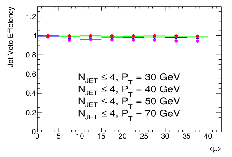
\includegraphics[width=\linewidth]{Znunu_mu_4jets_M0}
    \caption{No JVT cut applied.}
    \label{fig:znunu_4jets_jvt64}
  \end{subfigure}
  \begin{subfigure}[t]{.48\linewidth}
    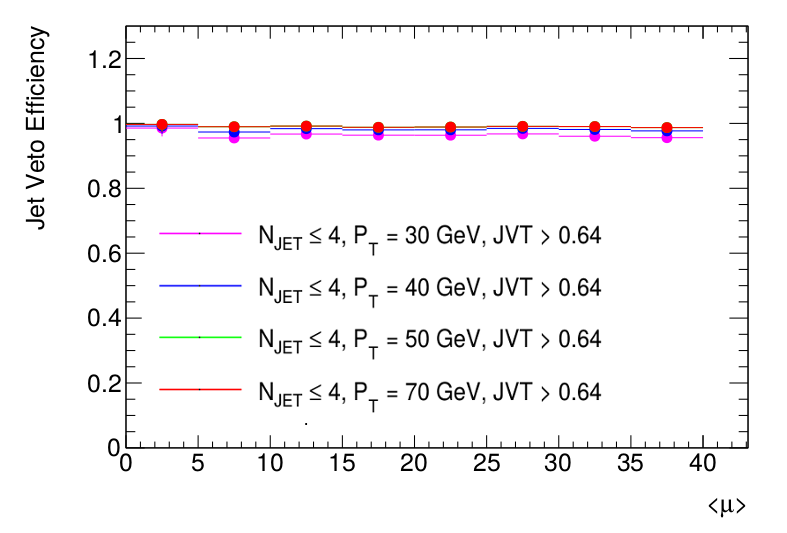
\includegraphics[width=\linewidth]{Znunu_mu_4jets_jvt64_M0}
    \caption{JVT > 0.64.}
    \label{fig:comp_4jets_jvt64_1}
  \end{subfigure}
  \caption{Jet veto efficiency for different jet $\pt$ thresholds and N (jets)
    $\leq 4$ as a function of the average number of interactions per bunch
    crossing $\langle \mu \rangle$ for the $\znunu$ background. In
    \cref{fig:comp_4jets_nojvt} no \gls{jvt} cut is applied and there is some
    drop of the efficiency at high pile-up. In \cref{fig:comp_4jets_jvt64} a
    \gls{jvt} $> 0.64$ cut is applied, the dependence from pile-up is reduced.}
  \label{fig:jet_veto_comparison}
\end{figure}
%%% Local Variables:
%%% mode: latex
%%% TeX-master: "../search_for_DM_LED_with_ATLAS"
%%% End:
